\chapter{Story Lane Theater 4}

% \begin{figure}[H]
%     \centering
%     
\includegraphics[width=\textwidth/2]{./Games/WriteAway/Images/WriteAway2CD.jpg}
%     \caption{Write Away 2 CD}
% \end{figure}

The fourth of the Story Lane Theatre games published and released by The Lightspan Partnership for the PlayStation 1.

Story Lane Theatre 4 features two video programs:

\begin{itemize}
    \item Following the Drinking Gourd
    \item King Midas and the Golden Touch
\end{itemize}

\clearpage
\newpage

\section{Following the Drinking Gourd}

\subsection{Audio Summary}

Follow the Drinking Gourd is a compelling tale based on a traditional folksong that celebrates the underground railroad and the perelous journey undertaken by slaves seeking to be free. The story is told by Morgan Freeman, with music by Taj Mahal. Backstage Pass visits with the illustrator, Yvonne Buchanan.

\subsection{Transcription}

Come on in, settle back. It's curtain time at the Story Lane Theater. You've never seen a stage like this one. Anything can happen.

Here, get ready for a journey. Look up at the stars to find your way. Today we'll be traveling with Mary Prentice and her family who are guided by a mysterious stranger named Pegleg Joe. But before we set out, let's go to Brooklyn, New York to meet Ivon Buchanan who made the paintings that brought all these characters to life.

"I grew up in New York, born and raised here. Moved out to Brooklyn about 12 years ago, graduated from Parsons. I always loved drawing, and when I was in sixth grade, my mother asked the teacher, Mr. Gibbons, if I could earn a living with art because she was very concerned about me being able to support myself, so once he said yes, she can earn money drawing, then it's like I was let free to do all sorts of things.

"I do most of my work at home. I have a studio separate from the rest of the house that I have my drawing table, my paints, and I work in there. When I started doing the drawings for Drinking Gourd, I realized I needed a lot of research. I needed to know about what kind of carts they used, what the houses looked like, what the clothes looked like, so I went up to the Schomburg Library, which is in Harlem, and I got a whole batch of pictures about plantations, farms, the type of brooms that women used, the kind of dresses they wore, hats, boots, type of landscape that the story took place in, just so that I can get an authentic feel.

"I felt I had to do the story justice because it tells the story of a little black girl, and I'm a black woman, and it's a very important story. I felt it touched me. I wanted to do a good job on it because of my family, you know, what my family had gone through.

"When I read the script and I got to know Mary, I went through a lot of different images of her. I started making her much more expressive instead of her being a passive little girl, feeling that she had more personality, and I just chose her eyes, large and slightly curved, and eventually I came up with this, and I realized that this drawing looks a lot like my sister, and here she is.

"Illustrators usually draw people they know. As you're growing up and you're learning how to draw a face or hands, you use your parents, you use your brothers and sisters as models, and so a lot of times you'll see a drawing of someone made up that actually looks like someone's parent or someone's sister.

"The story concerns a little black girl being strong, which you don't really see a lot of. When I was 9 or 11, I wasn't out in the field, I was in school. This little girl was forbidden to learn how to read, forbidden freedom, forbidden to play. She had to work like an adult, really not knowing whether anything was going to be all right, hoping that it will, but not really knowing.

"The character Pegleg Joe is a legendary character, and so I didn't want to depict him as a person particularly, but more as a mythic character, and so I wanted him to have lots of color in his beard - the greens, the pinks, and the reds of his beard that no human person has, because I think of him as a magical person who helped spirit this family away through the Underground Railroad.

"The central message the story tells is perseverance; courage. This picture takes place when Mary's mother is telling Mary and Samuel about the North Star, the Big Dipper, the Drinking Gourd, and explaining, you know, 'You follow the North Star to freedom, and this is how you get North.' What I wanted to show was hope in the mother's face and a little bit of apprehension in the children.

"I feel like the power in the story is that all these people - Mary, her mother, her brother - are all ordinary people who achieve extraordinary things, and I feel like everyone who feels that they're ordinary can achieve awesome things. So if you like to draw, you should draw every day, if you like to dance, you should dance every day, if you like science, you should learn about different formulas, learn about rocks, you know, whatever you're interested in. Each day learn something new, and you realize that (it will just) give you so much power in your own life."

And now we're ready to meet Mary Prentice and find out what it means to Follow the Drinking Gourd.

Twilight's just fallen. The day's cotton's been counted and carted, and out in the night just past the willow tree, you hear the quail whistle out to you. And that song sprouts up at the back of your throat about following the Drinking Gourd, about Pegleg Joe, about escaping North to freedom. But much as you want to sing it, you don't say a word. You just think it: Follow the Drinking Gourd. It's time to run.

Mary Prentice was only 11 years old when her mama decided to escape. See, Mary, her mama, and her brother Samuel were slaves on the Darby cotton plantation in a little town just outside Mobile, Alabama. Their papa used to be there with them, except he'd been sold when Mary was only 6 years old. So as it was, all three of them picked cotton, even Mary, six days a week. It was hard work, tiring work.

There was something special about Mary. She had a peculiar knack for gathering stories. She had ears sharp enough to pick up even the quietest whispers that might be floating about. One evening right after dinner, Mary snuck down to the stables. She probably should have been helping mama with the evening chores, but that night she was extra curious because she'd heard mention about Mr. Darby sending some of the slaves to auction.

The stable was an awfully dark and drafty place to visit at night, and what with all the rows of stalls and nooks and crannies for the feed and the tack, it seemed like an enormous maze. When Mary got there, the stables were quiet, but it didn't take long for her to overhear some stable hands whispering down at the far end of the stalls.

"Going to send five slaves, that's what I heard Mr. Darby sayin'. I even heard tell they'd be sellin' the Prentice boy as well."

Mary's face grew hot as an iron, but she stayed tight against the bin. Maybe she'd heard wrong. She wanted to run up and ask them, but they'd just shoo away a little girl like her. The voices grew softer and then shut off immediately when someone started banging hard on the padded gate.

Why had the men stopped talking? Mary ran to see who would be making that kind of noise.

It was a wild-looking fellow, and he was hammering away fast and hard, but it didn't look like he was getting too much work done. Mary hung back a little to watch him. He was what they like to call a journeyman because he traveled about doing carpentry and smithing. He had rough clothes, a mass of curly hair, and on his right side, a peg leg.

Mary's mind was swirling with the news about Samuel, but she couldn't help watch the man. Even above all the noise he was making, he kept singing the same little song: "When the sun comes back and the first quail cries, follow the Drinking Gourd. For the old man is waiting for to carry you to freedom if you follow the Drinking Gourd."

Mary was about to creep back to see if she could hear more from the stable hands when she saw Mr. Darby coming down the path. So quickly and quietly, she whisked herself away. Before she left, Mary took one last look at this peg-legged man, and maybe she was seeing funny, but it really looked as if he'd winked right in her direction.

Mary ran down the path to home - her feet shooting up dust and her mind heavy with the news about Samuel. Before she knew it, she was singing that song. She must have sung it a good 20 times when Mama clamped her hand right smack over Mary's mouth.

"Mary Prentice, where'd you go learnin' that song?" Mama's eyes were staring at her brighter than Mary had ever seen them.

"Song, Mama? Why, I just sort of picked it up from that peg-leg journeyman working in the stables. Did Papa ever talk about a journeyman like that? He sure was odd. Over and over he wouldn't sing nothing else."

That night Mama took Samuel and Mary out to the willow tree, out where nobody could hear, and she held them close to tell them about the song of the Drinking Gourd.

"Look up to where you see the big Drinking Gourd, up there overhead." Mama looked up at the stars and pointed to what they sometimes call the Big Dipper and sometimes the big Drinking Gourd, since it looked just like the big gourd they drank water out of when they worked in the fields.

Mama went on, "Now follow it with the little Drinking Gourd just beyond it. And right there at the tip of the handle, you can see that star shining bright like it's lookin' right towards you. That's the North Star."

Mary stared up at that North Star like she was trying to memorize it while Mama explained that the peg-leg man was called Pegleg Joe, and that he wasn't just a carpenter passing through town. He'd known Papa, and he was an agent for the Underground Railroad. So maybe Pegleg Joe's wink wasn't just her imagination. But did this mean that Mama was talking about escaping North? About them escaping North?

Mama's voice was hushed and serious. "'The old man is awaiting,' that's Pegleg Joe himself. He'll be the one to help us cross the river into the North. 'When the first quail calls' means the best time to go is spring. The weather's right, the river's high. 'Left foot, peg foot, traveling on,' we'll be following Pegleg Joe's path. Big leg on the right, footprint on the left."

Mary so wanted to ask the one question that kept biting at her: does this mean she might see her papa?

"The river bank makes a very good road. The dead trees will show you the way. Left foot, peg foot, traveling on, follow the Drinking Gourd. The river ends between two hills, follow the Drinking Gourd. There's another river on the other side, follow the Drinking Gourd. When the great big river meets the little river, follow the Drinking Gourd. For the old man is waiting for to carry you to freedom, follow the Drinking Gourd."

Next day, Mary's mother handed her something in a small red cloth and told her to run to the stables and give it to Pegleg Joe. Mary didn't know what it was, but she knew it would be their signal to say that they were ready to go. There he was, hammering away in the same place he'd been before. At first, he paid Mary no mind, and Mary wasn't sure that they could really trust him.

"The river bank makes a very good road, the dead trees will show you the way. Left foot, peg foot, traveling on, follow the Drinking Gourd."

Pegleg Joe kept right on banging on the gate, but Mary drew up close. The hammering grew softer, so she asked him, "But how do we get to the river?"

"Your mama knows."

"My mama knows no such thing. She's never left the plantation," said Mary.

"Your mama doesn't say all she knows, but she's got a map of the route right in her head, only she's going to need your help. Now your Papa's told me about you, and he said you as brave as they come and that you had enough stories in that head of yours to fill a shelf of books."

Her papa? Had Pegleg Joe seen him? Mary would have jumped up to ask all about it, only Pegleg Joe's eyebrows tightened together, and he began hammering harder than ever, and out of the corner of her eye, Mary could see that Mr. Darby was heading right down and towards the stables.

As she rushed to get to the back gate, she dropped the cloth, and out of it fell a small wooden object about the size of her thumb. It was a tiny Drinking Gourd, and Mary knew, looking at it, that Papa must have whittled it himself. There wasn't time to run back, so she tossed the little gourd straight back to Pegleg Joe and waited to watch him catch it.

Before long, she was back on the path to home, but she was sure she could hear Pegleg Joe say, "I'll be seeing you at the river."

That very night, Mama brought Mary and Samuel back out to the willow tree and wrapped them up in extra sets of clothes. Not a single word came across Mama's lips, but Mary knew that this was it. It was time to run.

Mary took a good look at the North Star to make sure it was looking out for them, and off she went, one step behind Samuel and two steps behind Mama, who carried only a cotton sack of food and the great big walking stick Papa had carved for her.

They had to get to the Tombigbee River before dawn to hide their trail. When Master Darby found them missing, he was sure to set out with the hunting dogs. Mary's legs grew tired. It seemed like Mama and Samuel were running. Mary crouched down on a stone to rest, but Mama shook her awake. She gave her a biscuit from the sack and rubbed Mary's feet. They were sore and blistered.

When they made it to the river, the sun was beginning to rise, and Mary could hear cocks crowing from a nearby farm. Mr. Darby would notice soon that they weren't in the fields. At the riverbank, Mama pointed to the ground with her walking stick. "Left foot, peg foot." There were Pegleg Joe's marks left for them to follow.

That day, and for many days, they traveled the riverbank at night and hid during the day in nearby swamps and marshes. They followed Pegleg Joe's footprints until at one bend in the river, the prints disappeared. They still had the Drinking Gourd as their guide, but each day they grew more tired and hungry, and they ate less and less as the food began running out.

That was when they decided that Samuel and Mary would hide out by the nearest plantation to see if they could get more food.

"If we are where I think we are, you'll find the slaves' quarters right next to the barn. Wait by the barn, and when it's pitch dark, you make the quail's call, nice and soft. And if you see a lantern light up in the slaves' quarters' four-paned window, there'll be someone to help you," said Mama.

Mary and Samuel waited until night to run. They hid by the barn and tried singing like the quail. No light came on, so they waited and waited. When it was so dark that they could barely see each other, sure enough, they saw a hand light a tiny lantern in the four-paned window. They leaned themselves hard against the barn, and before long, someone handed them a heavy cotton sack.

Mary could see only the outline of a very old face and a man bent over with age. "They've seen you, Mary and Samuel," the man's voice was a whisper.

"How'd you know our names?" asked Mary.

"There are posters up all over town. Your master's been sending out the alarm up the whole river."

"But where do we go if we can't use the river?" Samuel asked.

"There's pepper in the sack. Shake it after you if the dogs are near. It gets them off your trail. And follow the Drinking Gourd. If you make it past this stretch, you'll only have a few more days of following the river. And when you reach the Tennessee, there are good people there. Quakers. They'll know you're coming. They helped your papa."

"How will they know?" She waited to hear more, but there was no answer. The old man was gone.

Mary, Samuel, and Mama took to the woods. The river was no longer safe. They moved slowly, fighting against the vines and undergrowth. It didn't help to think that there were people after them ready to catch them for money. Mary and Samuel shook the pepper behind them, and as much as she hated the murky water and squishy mud, Mary wished she were back by the river.

Mary was first to hear the dogs. Mama said to pay them no mind, that they might just be chasing rabbits. But as the barking came closer, the three knew they'd better do something. The river was too far to run back to, so Mama threw the rest of the pepper onto the ground and pulled Mary and Samuel into a cascade of hundreds of kudzu vines. There was a small hollow place just large enough for them to crouch into.

The three of them squatted low and so close together it was hard to tell one heartbeat from another. Mama gripped them tight. The dogs were getting close, barking louder, faster, as if they knew just where the three were. Before long, there were voices with brusk voices coaxing the dogs on. "One thousand dollars for the boy! Come on, dogs! Track 'em down!"

Mary waited, sure they were caught. She could hardly believe it when the dogs stopped barking and started to whine. The pepper had worked. She saw Mama's mouth loosen into a smile.

A few days later, Mary, Samuel, and Mama came up a clearing in the woods, and beyond it, a small town. It surely wasn't a place that the three of them could walk into. In fact, there were probably posters right there with descriptions of them. But there, on the other side of the town was the Tennessee River.

That night, the three of them slipped through the clearing like cats. Then Mary heard something. Footsteps, and they were close. The three darted over to a cemetery and hid behind the biggest tombstone they could reach, but the footsteps kept after them.

"Art thou not Esther Prentice?" Mama didn't say a word, but Mary saw her lift up her head slowly. It was a Quaker man. He had a neatly trimmed beard shaped just along his jawbone. The man explained that they were in great danger. There were slave catchers looking for them all about the two rivers, the Tennessee and the Ohio. He said that if they could make it to his boat, moored just at the dock, then he could take them safely straight up the Tennessee River.

With Mama in the lead, they made themselves invisible, darting from building to building, crouching low and scarcely breathing. When they reached the boat, Mary's eyes opened wide with wonder when she saw the secret compartment under the deck. She and her family slipped down into it and listened while the Quaker man and his wife and son piled sack upon sack of flour and dry goods over the secret door.

That next morning, Mary and her family traveled up the Tennessee in broad daylight without even a single slave catcher guessing where they might be. The Quaker man warned them that their last stop, the Ohio River, was rife with patrols, and even Pegleg Joe couldn't guard against that.

As the song said, the river, that was the Tennessee, ends between two hills, and there's another river on the other side. It took days to find any trace of Pegleg Joe. It was Mary who spotted the prints: left foot, peg foot. And they raced to the end of the path to find a tiny inlet tucked into the hills. There they found more prints, but Pegleg Joe was nowhere to be seen. Mary felt her heart drop and her eyes grew hot with tears.

But then, to her amazement, out from behind the trees stepped Papa. Mary thought it was a dream, but Papa gripped her hand tight and placed in it the tiny Drinking Gourd. Papa looked tired, but he pulled Mama, Samuel, and Mary as close as he could and held on to them. Mary wasn't sure he would ever let go.

He said that all along the way, he'd heard about Mama and her two brave children, and that gave him the courage to run almost without stopping. There was lots to tell, but they still were not across the river. At nightfall, Papa took them by the hand and led them forward to Pegleg Joe.

When they reached the cove where Pegleg Joe's boat was hidden, there he was, waiting for them. The moon hid behind the clouds to let them cross, and the river frogs seemed to be croaking especially hard to wish them luck. Pegleg Joe rowed them across, soft and quiet as swans, right past the patrol, until the boat slowed and with a soft bump, they came to the other side of the river.

They still had a journey ahead of them until they were entirely safe, but this was it. They were together and on their way to freedom, and Mary could hear herself telling the story of their escape over and over in the days to come.

"The river bank makes a very good road,
The dead trees will show you the way.
Left foot, peg foot, traveling on,
Follow the Drinking Gourd.
The river ends between two hills,
Follow the Drinking Gourd.
There's another river on the other side,
Follow the Drinking Gourd.
When the great big river meets the little river,
Follow the Drinking Gourd.
For the old man is waiting for to carry you to freedom,
Follow the Drinking Gourd."

\subsection{Credits}

Told by: Morgan Freeman;
Illustrator: Yvonne Buchanan;
Written by: Bernardine Connelly;
Music Composed and Produced by: Taj Mahal;
Music Performed by: Taj Mahal (guitar + harmonica + banjo), Patrick Cockett (ukelele), Pancho Graham (electric + acoustic bass), Ben Harper (Hawaiian slide guitar), Kester Smith (drums and percussion);
Music Recorded and Mixed by: Michael Sena;
Narration Recorded and Soundtrack Mixed by: Chris Nelson;
Animation Camera: Gary McGivney;
Editor: David Russell;
Post Production: Palace Production Center (South Norwalk CT);
Series Logo Music: Jay Ungar;
Research and Development: Cheryl Carlesimo;
Editorial Director: Eric Metaxas;
Art Director: Paul Elliott;
Associate Producer: Doris Wilhousky;
Producer: Ken Hoin;
Director: John McCally;
Executive Producers: Mike Pogue, Mark Sottnick;

\section{King Midas and the Golden Touch}

\subsection{Audio Summary}

King Midas and the Golden Touch is a poinant adaptation of the Greek myth, that teaches that some things in life are more precious than gold. The story is told by Michael Cane, with music by Ellis Marsalis and Yoyoma. Backstage Pass visits with writer Eric Metaxas.

\subsection{Transcription}

Come on in, settle back. It's curtain time at the Story Lane Theater. You've never seen a stage like this one. Anything can happen here.

In a few minutes, we'll see "King Midas and the Golden Touch", but first, come on backstage to meet Eric Metaxas. He wrote the words for the story. This is Eric's favorite place to write. Let's listen to Eric tell how he goes about creating a story.

"The process of writing usually starts way before you actually pick up the pen or sit down in front of the word processor. Usually when I write, I'm writing a story in my mind before I'm actually writing it down on paper, I'm beginning to put it together and beginning to try to get the themes and the ideas of what I want to say, and in a way I'm editing the ideas in my mind, and then I'll sit down and I'll already sort of know what I want to say, so I'll just sit down and I'll write. Then when I'm finished, maybe a day later, I'll go back and I'll reread it and I'll realize that 'oh, there's all kinds of stuff that I wrote down that I didn't say as well as I could say it,' so I'll rewrite this paragraph and I'll add a few sentences here where something's not clear, and I'll get rid of this whole paragraph that I wrote yesterday because it's not really saying what I wanted it to say.

"One of the reasons that I was so eager to write the story of King Midas is because it's a Greek story and because I'm Greek, and we can trace my relatives back 540 years in the very same place on the island of Cephalonia, the Maxis family has been there and actually have a picture of some of my relatives. This is my great-grandfather [Panagiotis (inaudible)] and that's his wife Eleni. This is my grandmother Rene and her twin sister Angeliki.

"[Panagiotis (inaudible)] was a writer. He made his living as an educator, school principal, and he wrote a lot of books, and my father always kids me that that's sort of where I get my writing talent from, from [Panagiotis (inaudible)], that it's his genes. But my father also tells me that his wife Eleni, when she was older, she was a real storyteller, that she would tell the neighborhood kids stories and my father, of course, remembers sitting with the neighborhood kids at her feet while she would sort of spin a yarn, and I've got another picture of her here when she was a little bit younger, probably about 19 years old. She was quite a storyteller too, so in a way, we have two different kinds of storytellers in my family - we have the oral storyteller and we have the writer.

"In the story of King Midas, there's something that I put in because it's very similar to what happened to me when I was in Greece. When I was in Greece, everybody went to sleep during the afternoons because the sun was so bright and so hot. But when I was there, I didn't. I kind of enjoyed the fact that everybody had gone to sleep and I could sort of walk around and it was really peaceful, and I felt like I had the whole world to myself. And in the story of King Midas, both King Midas and his daughter, Zoe, they also stay up during the afternoon because it's really quiet, and there's a line in the story about where Zoe enjoyed the afternoon so much that she didn't like to go to sleep, so I put a little piece of myself in Zoe when I was writing the story.

"A lot of times when I'm having problems putting pen to paper and I'm at a sort of a rough spot in the writing process, I'll just want to get away from everything for a few minutes. A lot of times I'll take a walk and I usually go to a park that's near here which is really, really beautiful and there are very, very few people there, and so in a lot of ways it reminds me of the afternoon walks I used to take when I was in Greece, because you feel like you're the only person in the world and you can be completely alone with your thoughts.

"Sometimes when I'm in a place that's as beautiful as a place like this, it really amazes me that there's really nothing that you could do to improve upon it. It's so beautiful that the best thing you could possibly do is to try to take it in, to try to appreciate it for what it is, and I think in the story where King Midas goes wrong is that he's not content with what he has. He really seems to think if he could just do one more thing, if that beautiful butterfly could just be golden, then he'd have everything he wanted. But sometimes if you're not content with the beauty of things, with the beauty of the water and the beauty of the flowers, and being with the people that you care about, and you reach for that one thing to try to make it better the way King Midas did, you sort of can ruin everything, and that's really what happens to him in the story and everything that he had, the beauty all around him sort of gets destroyed and he learns a painful lesson that there are many things in life that are worth a lot more than gold."

Thanks for sharing those thoughts with us, Eric, and now let's watch King Midas and the Golden Touch.

Once upon a time, about 27 centuries ago actually, somewhere on the coast of what is now Turkey, there was a sunny kingdom called Phrygia. For many years, the ruler of this kingdom was a certain King Midas.

Now King Midas was a very wealthy man. Indeed, he had everything money could buy. But of all the things he possessed in the world, he valued nothing more than his only daughter. She was as dear to him as life itself, and it was for this very reason that he named her Zoe, which means life.

Because the sun is very strong in Phrygia, most of the people who have ever lived there prefer to sleep during the afternoons and do their work during the cooler hours of the morning and evening. But it was precisely during those hot afternoon hours that King Midas's daughter loved to play most, and so dearly did the king love his daughter that he could not refuse her this wish. So as his servants slept, he would contentedly sit and watch her play from the cool shade of his grape arbor, which overlooked his magnificent gardens, which in turn overlooked the brilliant blue sea.

And during many of the long sleepy afternoons in which he sat watching her run about chasing birds and smelling flowers, it was King Midas's particular habit to carefully count out some number of the gold coins that he possessed. There was quite a large number of them. In fact, he never could have counted them all, and each and every one of them, large and small, was exquisitely minted with the king's own regal profile. The likeness was perfect to the very tiniest detail, and had it not been for the small cosmetic addition of the six-rayed crown of the sun god Helios, with whom in his heart of hearts good King Midas liked to be identified, one might have easily mistaken the miniature golden image for the very king himself.

Now one day as he was sitting there in the arbor counting his coins, the king observed his daughter following a beautiful white butterfly as it flitted lazily down one of the garden paths. The butterfly was so marvelously delicate as to be almost transparent, and as King Midas watched it, he could not help but admire the exceptional freedom and beauty of the creature. But as he beheld it, the strong rays of the Phrygian sun came to illuminate it in such a way that for some time as it floated before him, it seemed to him to be made entirely of gold.

The sight of this had the power of revelation, and it so completely transfixed the king that long after the butterfly had flown out of his ken and on its way, he remained staring at where it had been as though under a powerful spell. And when he came to himself again, he remained consumed with the idea of it. A butterfly made of gold. Astounding. I've never seen anything as beautiful in my life. I simply must have one. A butterfly made of gold.

Now the idea of wanting a golden butterfly seemed at the time to be quite harmless. After all, he only wanted it to be able to give it to his daughter. But as he ruminated further on the great beauty and worth of such an object, his small wish for a golden butterfly blossomed into an overwhelming desire that everything in the world might become gold. How beautiful the world would be if all things could be transformed as magnificently as the butterfly had, he thought to himself. If only I had the power to accomplish it. I should give anything to have that power. Anything at all.

His obsession with this thought did not leave him for several weeks, but one day, when the wish became so fervent that he thought he couldn't stand it another moment, the king looked up and saw a golden chariot descending towards him out of the bright sun. The curious being who debarked from it was dressed entirely in gold and claimed to be a messenger of none other than Helios the lightbearer himself.

"Your most fervent wish has been heard, good King Midas," he said, "and it is our majesty's equally fervent wish that it should be granted. Therefore, as soon as the sun rises tomorrow, you shall possess your desire, for as you will then perceive, all that you touch from that time forth shall turn to the purest gold." Then with a flourish of his hand, he conjured a brilliant box which he said contained a golden piece of the very sun itself. "A small gift for the good king," he said. "For the good and great King Midas."

Naturally, King Midas was deeply impressed, but when he reached out to touch the gift, it burned his hand. "Ah yes," said the odd man with a queer smile. "Perhaps such a gift wasn't meant for your kind after all." With that, he climbed back into his gilded chariot and again ascended into the blinding brilliance of the afternoon sun.

Of course, all this made the king quite eager for the next day, but when the sun's first rays entered his chamber in the morning, he became terribly uncomfortable. He tossed and turned endlessly about in his bed, but he was unable to find another moment's peace, and was at some point soon thereafter that he came to realize that the very bed upon which he lay was made entirely of gold.

Now as you will doubtless understand, the king's joy at this realization can hardly be described, and the small price of a few hours of lost sleep was simply unworthy of comparing with the exquisite joy he now felt. Oh, he was elated!

It next occurred to him that the odd messenger's promise must have come true and anything he touched might now turn to gold. Without a moment's hesitation, he was out of the bed and furiously looking about the room for a suitable object on which to experiment. He grew quite dizzy at the prospect of it all.

At last his eyes came to rest on an ornately carved chair. He immediately moved toward it and then, ever so cautiously, he touched it. Instantly it was transformed into a chair of the purest gold. On examining it more closely, King Midas saw that every part of it had been transformed - the upholstery, the carved wood, even the braided tassels that hung from it were gold. He could hardly believe his eyes.

But the remarkable metamorphosis only seemed to whet his appetite for more. He saw a table just outside his bedchamber and he touched it. He touched the tapestry. Then as fast as his legs could carry him, he ran into the garden. He touched a marble statue, a vase, and everything he touched, every single thing turned to gold. It was more than he could bear.

Then King Midas stooped to pick up a white pebble and no sooner had he touched it than it was gold. He saw another stone slightly larger and touched that, and it too became gold. The king next spotted a large conch shell that his daughter had discovered on the seashore. He remembered the day she had found it and recalled holding the shell to her ear so that she could hear the sounds of the ocean inside it, and how she heard it saying "Thalassa, thalassa, thalassa" like the waves of the sea. In a flash, he touched it and it too was transformed to gold before his very eyes. It was magnificent.

He lifted the golden conch to examine it and hold it to his ear, unable to imagine what golden music should come out of it now. But he found that it was extremely heavy, and when he held it up to his ear, he heard absolutely nothing. Now normally this would have saddened King Midas, but under the circumstances, his thoughts turned rather quickly to the subject of what other objects he might turn to gold.

In a moment his attention was captured by a beautiful flower, and when he touched it, the leaves, the stem, every petal, and even the intricate universe within the petals turned to gold. He quickly touched another flower and then another and another. It was all too much to behold.

Then King Midas saw a white butterfly. It was quite like the one that he had so admired some weeks before, and as he was powerless to do anything else, he began to chase it. The chase took him down one garden path and then another until as carefree as a small child, he completely lost track of himself.

The butterfly eventually led him along the very edge of the castle parapet overlooking the ocean, and because the idea of having a golden butterfly consumed him so completely, he quite forgot about the long drop to the rocks below and continued to chase it, teetering along the edge of the parapet as the butterfly danced just out of his reach. At last, reaching so far out that he nearly fell, the king succeeded in grazing the creature's gossamer wing with the tip of his outstretched index finger. But on the very instant that he did so, it stiffened to gold and fell away out of his reach, down, down it fell all the way to the seawash rocks below where it hit with a dull plink and disappeared among the barnacled crevices - a lifeless bob.

King Midas stood there staring at where it had fallen, unable to believe what he had just seen. He had never considered that he might kill the poor creature.

As he wound his way back to the palace, King Midas passed several ancient olive trees, and tired from his chase, he leaned up against a particularly venerable specimen. As soon as he touched the trunk of the great tree, however, everything above him and around him froze into a single golden moment. It was an extraordinary sight. The entire tree, its mammoth gnarled trunk, every branch, every oval leaf, every green olive had turned to gold.

King Midas saw that even the hundreds of ants and other tiny insects on the tree had turned to gold. He beheld a golden inchworm frozen in the act of measuring its last inch. There was a golden nest of golden eggs that would never hatch and a golden hive of bees that would never produce honey again. Then in a remote branch of the tree, he beheld the dazzling tracery of a golden spider's web and finally a long descending strand of golden spider silk and the attached arachnid who had spun it and would spin no more.

When he finally returned to the palace, he called to his servants to prepare a banquet and cheerily announced to them that it would all be on plates of gold. Although they were quite puzzled, they complied with his request, and no sooner than they had set a plate before him did he touch it and turn it into gold before their eyes. Everyone was completely astounded, but King Midas only laughed and performed his magic on the silver goblet that was set before him. He then proceeded to turn all the serving platters to gold as well as the very table on which they were placed.

But when the novelty eroded and King Midas at last decided to get down to the actual business of eating, a curious thing happened. You see, when he picked up a fig to put it in his mouth, it too turned to solid gold. And when he tried to pour himself a glass of wine, both the bottle as well as the liquid inside became gold. He then grew frantic, grabbing first a cluster of grapes and then a handful of olives, but to his great consternation, each and everything that he touched turned quite indisputably into an object of solid gold. The king became deeply distressed. He would soon starve.

Just then, the king's daughter came running out of the palace to greet him. King Midas was so delighted to see her that he quickly embraced her, but no sooner did he do this that he recoiled in horror, for the golden touch with which he had been lately cursed had worked its hideous magic even on his precious daughter whom he loved beyond anything in the world.

"Oh my Zoe!" he cried. "My dear Zoe! I have lost my dear Zoe!" In his grief, he began running, he knew not where. After a time, the king found himself at the edge of a stream. He sat down exhausted, and putting his face in his hands, he began to sob. "I have lost my Zoe," he cried. "I have killed everything that I have touched, and now I have killed the very thing in the world that was dearest to me. I don't wish to live. I don't care if I am the richest man in the universe."

But as he was crying, the king noticed an odd thing, for somehow the tears that were on his cheeks and in his hands hadn't turned to gold. Nor, inexplicably, had the stone upon which his hand rested. Was it possible?

As fast as he could, King Midas ran back to the palace. With great trepidation, he touched one of the flowers that he had turned to gold. In an instant, it became a living flower again. He touched another and another. "Oh, this is much too good to be true," the king thought. The king then ran to where his daughter stood. At the sight of her, tears came to his eyes again. Then with a trembling hand, he touched her cheek. Immediately, the warmth and color of life returned to her. The king immediately fell on his knees weeping with joy. He embraced the dear child tenderly.

"Oh my Zoe, my Zoe," he cried. "I have found my dear Zoe!"

And what the king said was quite true, for indeed he had.

That day, King Midas called a large feast. It was a celebration unlike anything the world had ever seen, even to this day. Every [lader] was empty and nothing was spared, not a single thing, for you see there was no earthly extravagance that could match King Midas's love for his daughter.

And when the celebration was over and everyone had gone home, King Midas instructed his servants to gather up all the golden coins in the treasury and bring them to the castle parapet. And there, as the sun dipped beyond the horizon, he and his Zoe, his beloved Zoe, tossed them out over the water one by one. And one by one, each of the golden coins was transformed into a beautiful white butterfly that flew up and up and up into the magnificent blue sky.

\subsection{Credits}

Told by: Michael Caine;
Drawings by: Rodica Prato;
Written by: Eric Metaxas;
Music Composed by: Ellis Marsalis;
Music Performed by: Ellis Marsalis (piano), Yo-Yo Ma (cello), Brian Blade (drums), Chris Thomas (acoustic bass);
Music Produced by: Delfeayo Marsalis;
Music Engineered by: Patrick Smith;
Narration Recorded by: Robert Norman;
Soundtrack Mixed by: Chris Nelson;
Editor: Mark Forker;
Assistant Editor: Anna Pivarnik;
Post Production: Rebo High Definition Studio (New York NY);
Art Consultant: Roland Caracostea-Balan;
Art Director: Tim Raglin;
Associate Producer: Doris Wilhousky;
Producer: Ken Hoin;
Director: C.W. Rogers;
Executive Producers: Mike Pogue, Mark Sottnick;

\clearpage
\newpage

\section{Screenshots}

\begin{figure}[H]
    \centering
    \begin{subfigure}{0.45\textwidth}
        \centering
        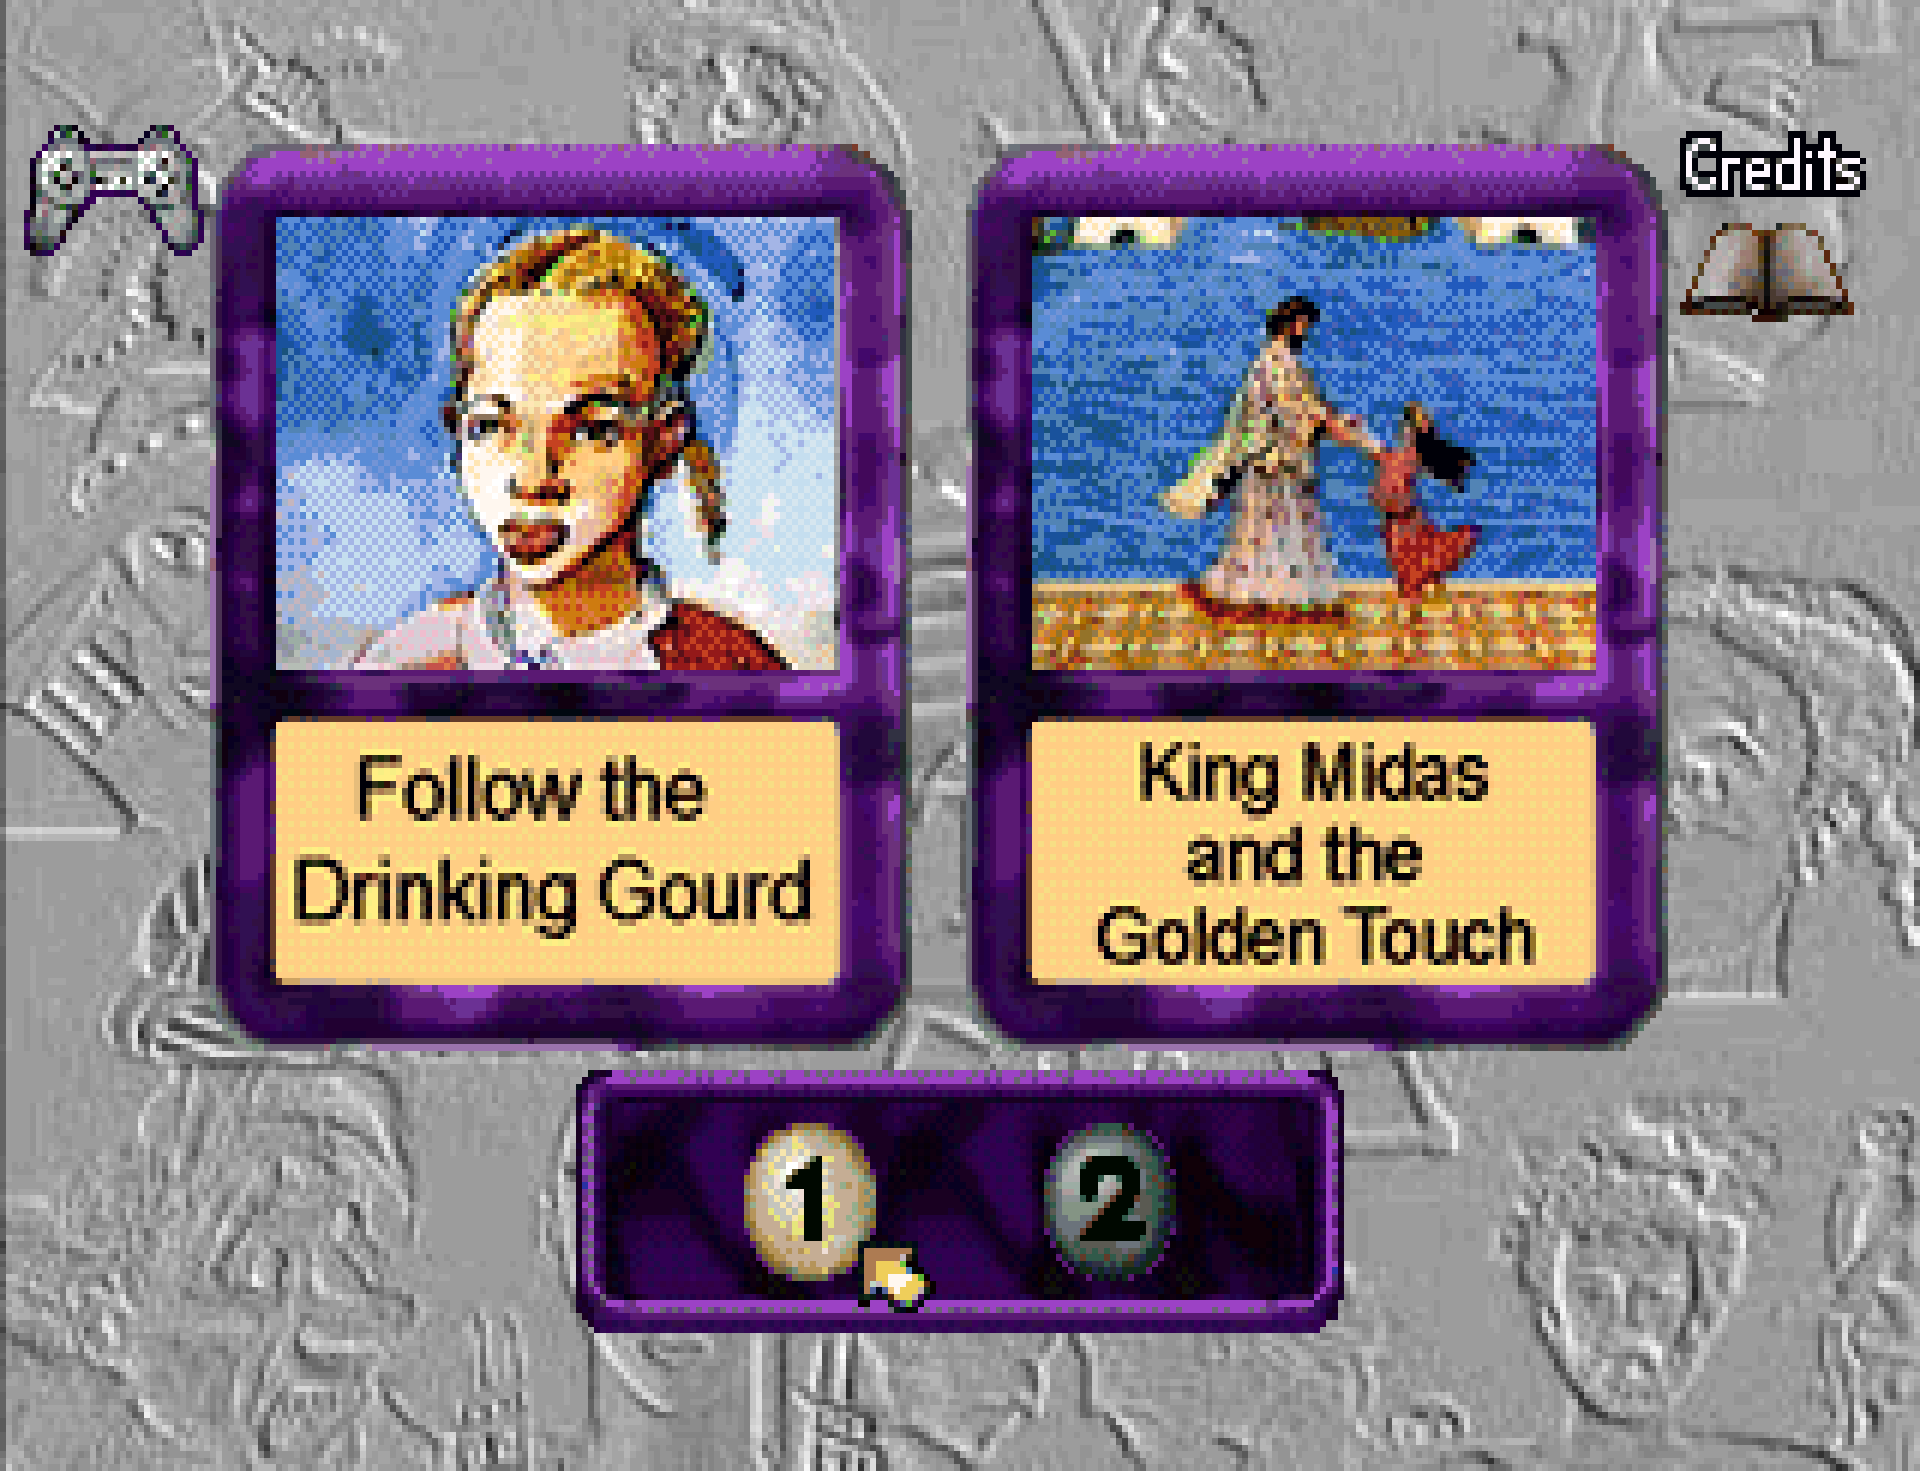
\includegraphics[width=\linewidth]{Games/StoryLaneTheater/Images/StoryLaneTheater4Image1.png}
        \caption{Story Lane Theater 4 - Screenshot 1}
    \end{subfigure}
    \begin{subfigure}{0.45\textwidth}
        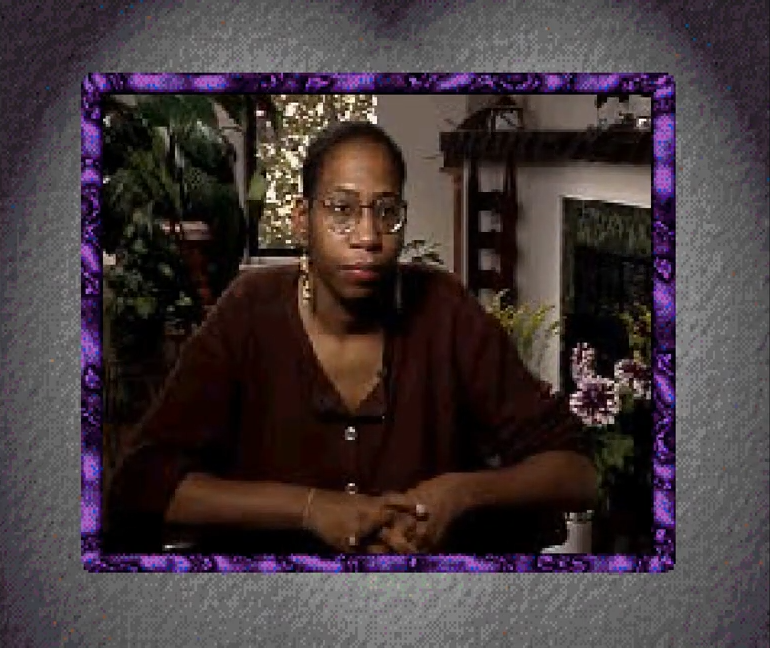
\includegraphics[width=\linewidth]{Games/StoryLaneTheater/Images/StoryLaneTheater4Image2.png}
        \caption{Story Lane Theater 4 - Screenshot 2}
    \end{subfigure}

    \begin{subfigure}{0.45\textwidth}
        \centering
        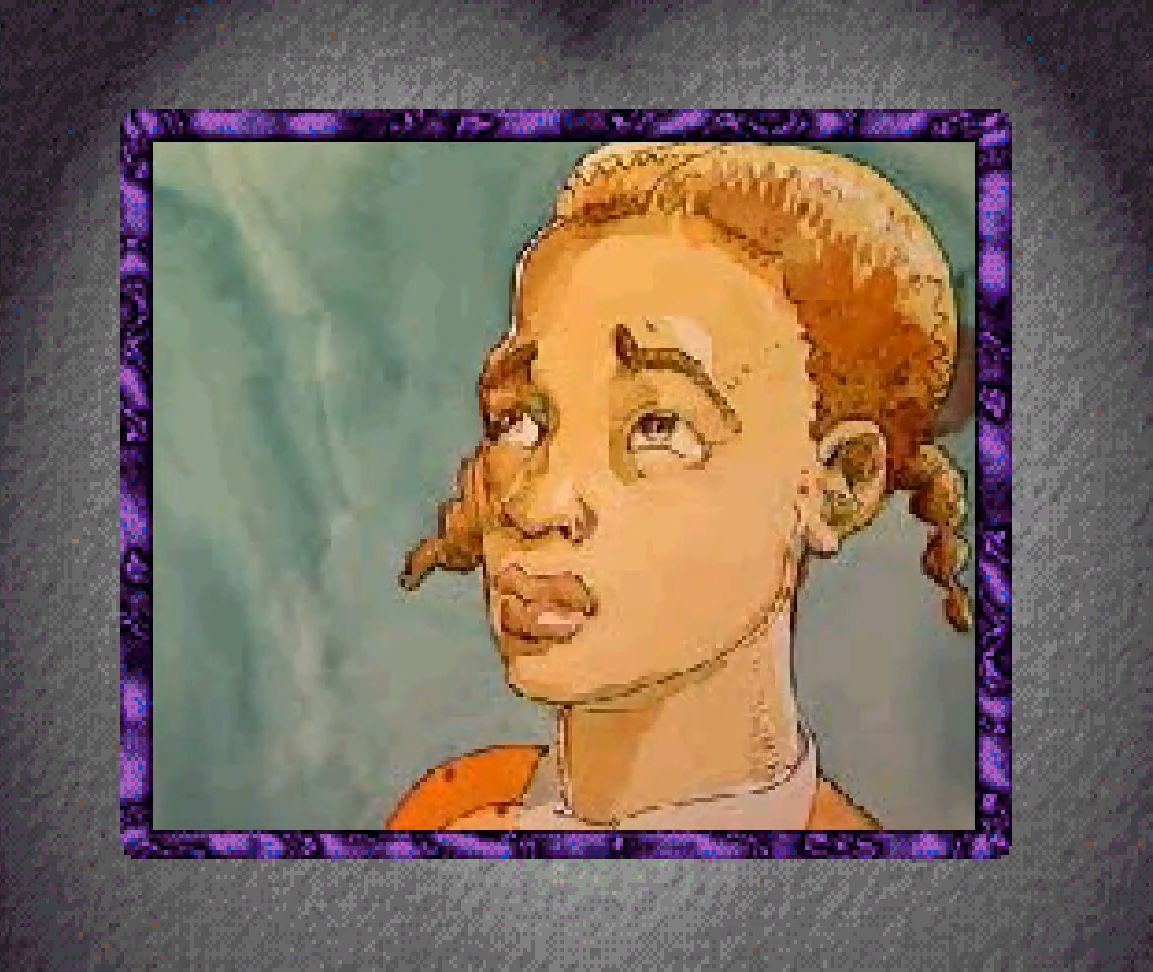
\includegraphics[width=\linewidth]{Games/StoryLaneTheater/Images/StoryLaneTheater4Image3.png}
        \caption{Story Lane Theater 4 - Screenshot 3}
    \end{subfigure}
    \begin{subfigure}{0.45\textwidth}
        \centering
        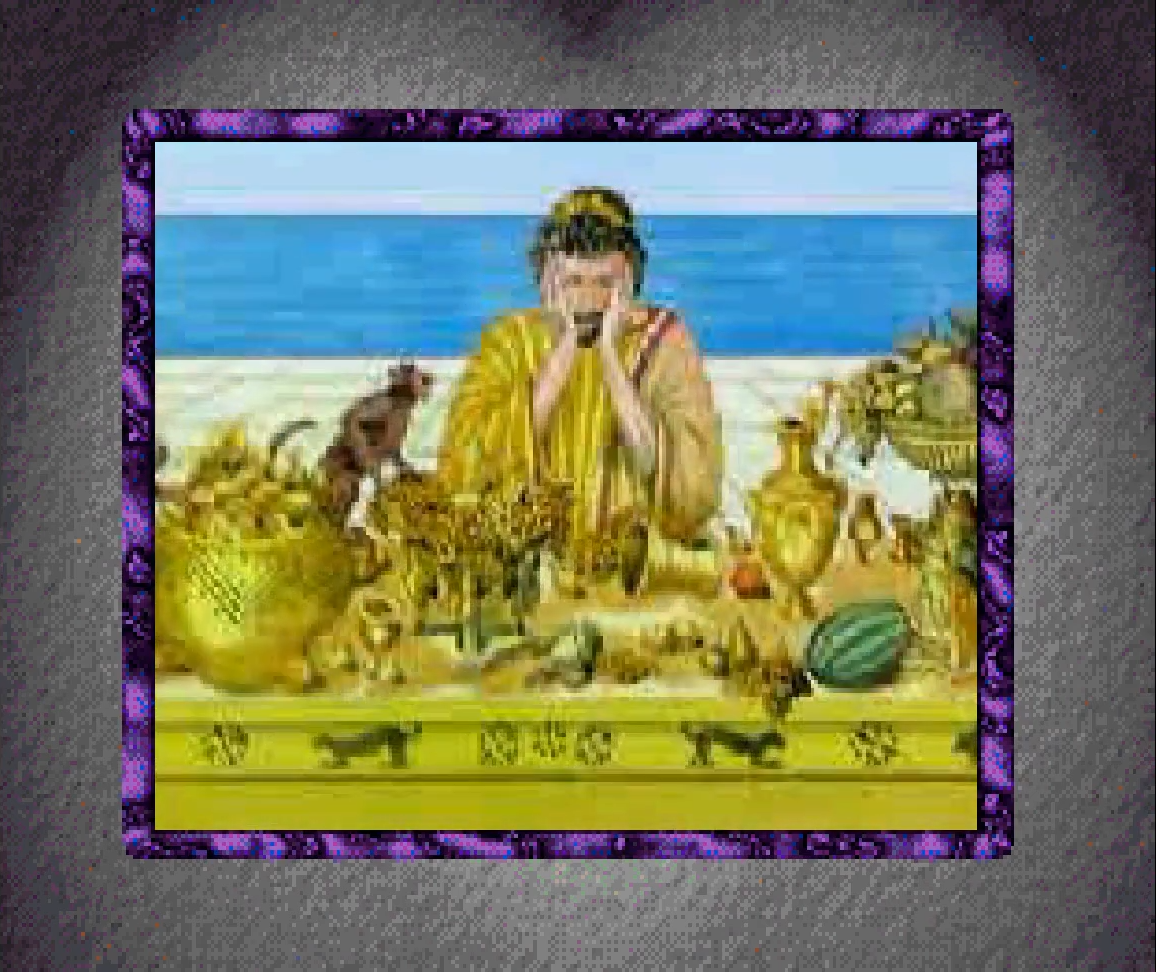
\includegraphics[width=\linewidth]{Games/StoryLaneTheater/Images/StoryLaneTheater4Image4.png}
        \caption{Story Lane Theater 4 - Screenshot 4}
    \end{subfigure}
    \caption{Screenshots from Story Lane Theater 4}
\end{figure}